
The contribution of this study on travel mode choice is the research on modeling choice behaviors in travel mode selection using game theory concepts, and using an evolutionary analysis to determine the behavior of the travelers.
\clearpage

\section{Evolutionary Game Theory and Travel Mode Choice}
Evolutionary game theory is used as a vehicle for discussing travel mode choice based on the following apparent similarities: 
\paragraph{}A group can be a substitute for an individual as a participant in evolutionary game theory, and the proportions of the individuals choosing different pure strategies in the group can substitute for mixed strategy. The results of travel mode choice are group behavior within the travel mode subsystems, and the only proportions of individuals choosing each travel mode are meaningful for management and study.
\paragraph{}Nash equilibrium means that the frequency of the adopted strategies makes the strategy payoffs exactly equal with no one desiring a change in strategy, then the percentage of individuals choosing each different strategy remains stable and reaches equilibrium. In the stable travel context, a travel mode choice will tend to be stable, the Nash equilibrium of the evolutionary game will be changed by the means of traffic control, the construction, and the structure of the transportation system.

\subsection{Evolutionary Game Model}

Inspired by the nested binary logit model used to define mode choice and Zhu et al (2018) study, the multi-agent based mode choice game is represented in extensive form in Figure \ref{fig:555}.
Players in the travel mode choice game are be divided into two main categories: car owners and noncar owners. First, every player chooses whether they own a car or not; then, the car owners will select from one of four modes: car, taxi, bus, or rail, and the noncar owners will only select from taxi, bus, or rail. Furthermore, two sub-games are apparent, a car owners sub-game and non car owners sub-game.

\paragraph{} As mentioned in Chapter 1, the extensive form is defined by the set of players, the strategy sets , and the payoff function.
\begin{itemize}
\item the set of players $N = {1,...,n}$, all travelers are players.
\item The strategy sets of the players are $S_1 = {Car owneer, Noncar owner}$ and $ S_2 = $(Travel by car, Travel by taxi, Travel by bus, Travel by rail).
\item The payoff functions of the players are $f_{car} = u_1$, $f_{taxi} = u_2$, $f_{bus} = u_3$, and $f_{rail} = u_4$
\end{itemize}
\paragraph{}Players use mixed strategy, because it is impossible for them to travel using the same pure strategy mode multiple times with certainty.
\paragraph{}As explained in Chapter 1, the mixed strategy happens when an individual plays one of the pure strategies of a game with a continuous probability $p$ between 0 and 1. As a result, the payoff the of the individual using mixed strategy depends on the probabilities of the mixed strategy.
\paragraph{}Figure 3.1 shows the game model of travel mode choice, we note that in stage 1 of the game $p_c$ and $p_n$ are the probabilities of car owners and non car owners respectively. In stage 2, $r^c_{c}$, $r^{c}_{t}$, $r^c_{b}$, and $r^c_{r}$ are the respective probabilities of car owner traveling by car, taxi, bus or rail. The probabilities of the noncar owner traveling by taxi, bus or rail are $r^n_{t}$, $r^n_{b}$, and $r^n_{r}$.
\paragraph{}The payoff function of the players are the following: 
\begin{equation}
f_{car} = T_{car} C_{car}
\end{equation}
\begin{equation}
f_{taxi} = T_{taxi} C_{taxi}
\end{equation}
\begin{equation}
f_{bus} = T_{bus} C_{bus}
\end{equation}
\begin{equation}
f_{rail} = T_{rail} C_{rail}
\end{equation}
\paragraph{}where travel time averages for car, taxi, bus, and rail are $T_{car}$, $T_{taxi}$, $T_{bus}$, $T_{rail}$, and their average travel costs are $C_{car}$, $C_{taxi}$, $C_{bus}$, $C_{rail}$ respectively.
\begin{figure}
 
  \centering
  \begin{tikzpicture}[baseline] % baseline makes the example number stay at the top of the tree
   \Tree[.N [.\textit{Car Owner} [.Car \textit{$U_1$} ][.Taxi \textit{$U_2$} ][.Bus \textit{$U_3$} ][.Rail \textit{$U_4$} ]][.\textit{Non Car Owner} [.Taxi \textit{$U_2$} ][.Bus \textit{$U_3$} ][.Rail \textit{$U_4$} ]]]
     \end{tikzpicture}%
  \caption{Travel mode choice game\label{fig:555}}
\end{figure}
\subsection{Nash Equilibrium of Travel Mode Choice Game}
According to the Folk Theorem mentioned in Chapter 1, any payoff vector satisfying individual rationality can be obtained through a set of specific subgame perfect equilibriums in an infinitely repeated game. In Figure \ref{fig:555} there are two subgame: Car owner subgame and noncar owner subgame, as shown in figures \ref{fig:3} and \ref{fig:4}.The Nash equilibrium of the game is a subgame perfect Nash equilibrium of each sub-game. As mentioned in Chapter 1, backward induction is the method for solving extensive form games and obtaining the Nash equilibrium.

\subsubsection{Nash Equilibrium of Car Owner Subgame}The key feature of mixed strategy Nash equilibrium is that the expectations of the pure strategies are equal, that is, in car owner subgame of figure \ref{fig:3}. \\

\begin{figure}[!h]
  \centering
  \begin{tikzpicture}[baseline] % baseline makes the example number stay at the top of the tree
   \Tree[.\textit{Car Owner} [.Car \textit{$U_1$} ][.Taxi \textit{$U_2$} ][.Bus \textit{$U_3$} ][.Rail \textit{$U_4$} ]]
     \end{tikzpicture}%
  \caption{Car owner subgame\label{fig:3}}
\end{figure}
The products of the travel mode's payoffs and its probabilities are equal and the sum of their probabilities is 1:
\begin{equation}\label{eq:8}
\mu_1 r^c_{c} = \mu_2 r^{c}_{t} = \mu_3 r^c_{b} = \mu_4 r^c_{r}
\end{equation}
\begin{equation}\label{eq:9}
\mu_1 r^c_{c} +  \mu_2 r^{c}_{t} + \mu_3 r^c_{b} + \mu_4 r^c_{r} = 1
\end{equation}

Solving \ref{eq:8} and \ref{eq:9}
\begin{equation}\label{eq:5555}
r^c_{c} = \frac{1}{1+ (\mu_1 / \mu_2)+(\mu_1 / \mu_3)+(\mu_1 / \mu_4)}
\end{equation}
\begin{equation}
r^c_{t} = \frac{1}{1+ (\mu_2 / \mu_1)+(\mu_2 / \mu_3)+(\mu_2 / \mu_4)}
\end{equation}
\begin{equation}
r^c_{b} = \frac{1}{1+ (\mu_3 / \mu_1)+(\mu_3 / \mu_2)+(\mu_3 / \mu_4)}
\end{equation}
\begin{equation}
r^c_{r} = \frac{1}{1+ (\mu_4 / \mu_1)+(\mu_4 / \mu_2)+(\mu_4 / \mu_3)}
\end{equation}

\subsubsection{Nash Equilibrium for Noncar Owners Subgame}
Using backward induction properties as explained in Chapter 1 to solve the subgame shown in Figure \ref{fig:4}. \\

\begin{figure}[!h]
  \centering
  \begin{tikzpicture}[baseline] % baseline makes the example number stay at the top of the tree
   \Tree[.\textit{Non Car Owner} [.Taxi \textit{$U_2$} ][.Bus \textit{$U_3$} ][.Rail \textit{$U_4$} ]]
     \end{tikzpicture}%
  \caption{Non car owner subgame\label{fig:4}}
\end{figure}
The products of the travel mode's payoffs and its probabilities are equal, and the sum of their probabilities is 1, resulting in: 
\begin{equation}\label{eq:10}
\mu_2 r^n_{t} = \mu_3 r^n_{b} = \mu_4 r^n_{r}
\end{equation}
\begin{equation}\label{11}
\mu_2 r^n_{t} + \mu_3 r^n_{b} + \mu_4 r^n_{r} = 1
\end{equation}
Solving \ref{eq:10} and \ref{11} 
\begin{equation}
r^n_{t} = \frac{1}{1+(\mu_2 / \mu_3)+(\mu_2 / \mu_4)}
\end{equation}
\begin{equation}
r^n_{b} = \frac{1}{1+ (\mu_3 / \mu_2)+(\mu_3 / \mu_4)}
\end{equation}
\begin{equation}\label{eq:666}
r^n_{r} = \frac{1}{1+ (\mu_4 / \mu_2)+(\mu_4 / \mu_3)}
\end{equation}
\subsubsection{Nash Equilibrium of Travel Mode Choice Game}
The payoffs of the car owner and the non car owner are their overall expectations. Using backward induction, the products of the payoffs and probabilities are equal and the sum of their probabilities is one: 
\begin{equation}\label{eq:12}
r_n(\mu_2 r^n_{t} + \mu_3 r^n_{b} + \mu_4 r^n_{r}) =  r_c(r^c_{c} + r^{c}_{t} + r^c_{b} + r^c_{r})
\end{equation}
\begin{equation}\label{eq:13}
p_c + p_n = 1
\end{equation}
Solving \ref{eq:12} and \ref{eq:13}
\begin{equation}
p_c = \frac{\mu_2 r^n_{t} + \mu_3 r^n_{b} + \mu_4 r^n_{r}}{\mu_2 r^n_{t} + \mu_3 r^n_{b} + \mu_4 r^n_{r} + \mu_1 r^c_{c} +  \mu_2 r^{c}_{t} + \mu_3 r^c_{b} + \mu_4 r^c_{r}}
\end{equation}
\begin{equation}
p_n = \frac{\mu_1 r^c_{c} +  \mu_2 r^{c}_{t} + \mu_3 r^c_{b} + \mu_4 r^c_{r}}{\mu_1 r^c_{c} +  \mu_2 r^{c}_{t} + \mu_3 r^c_{b} + \mu_4 r^c_{r} + \mu_2 r^n_{t} + \mu_3 r^n_{b} + \mu_4 r^n_{r}}
\end{equation}
\paragraph{}The proportion of travel by car for the traveler is the product of its probability and the probability of car owners traveling by car, and the same goes through other modes:  
\begin{equation}\label{eq:14}
\gamma_{car} = p_c r^c_c
\end{equation}
\begin{equation}
\gamma_{taxi} = p_c r^c_t + p_n r^n_t
\end{equation}
\begin{equation}
\gamma_{bus} = p_c r^c_b + p_n r^n_b
\end{equation}
\begin{equation}\label{eq:15}
\gamma_{rail} = p_c r^c_r + p_n r^n_r
\end{equation}
Substituting equations \ref{eq:5555} to \ref{eq:14}
\begin{equation}
p_{c} = \frac{\frac{3}{(1/\mu_2)+(1/\mu_3)+(1/\mu_4)}}{\frac{4}{(1/\mu_1)+(1/\mu_2)+(1/\mu_3)+(1/\mu_4)}+\frac{3}{(1/\mu_2)+(1/\mu_3)+(1/\mu_4)}}
\end{equation}
\begin{equation}
p_n{} = \frac{\frac{4}{(1/\mu_1)+(1/\mu_2)+(1/\mu_3)+(1/\mu_4)}}{\frac{4}{(1/\mu_1)+(1/\mu_2)+(1/\mu_3)+(1/\mu_4)}+\frac{3}{(1/\mu_2)+(1/\mu_3)+(1/\mu_4)}}
\end{equation}
\paragraph{}The equations above represent the Nash Equilibrium of the travel mode choice game. Looking through equations \ref{eq:14} to \ref{eq:15} we can see that there is a relationship between the individual's payoff and their proportion. That is, as its payoff is increasing, the proportion is decreasing. However, in the last four equations there is a relationship between the proportion and the payoffs of all the travel modes.
The essence of evolutionary analysis is to discuss how the probability changes when one side of the game changes. The learning ability of travelers, which is usually reflected by the tendency dynamic characteristics, in order to determine the change rate.
\section{Constructing the model}
This model is an agent based model of artificial agents playing the travel mode choice game. Each agent occupies a single place in the game and could interact with other neighbor agents. Agents in this game will update their state based on their game choices. An agent's state can be either a car owner or a non car owner which makes him a public transport user. If a non car owner switches their state to a car owner, they have to go through "purchasing a car" according to the probability function. This probability to buy a car function is adopted from an agent based computational approach (Epstein, 2002).
\section{Model Analysis}
\subsection{Travel Cost}
The cost of traveling is an important factor in TMC, although, travel time can be an affecting factor. Measures like public transport fares, car utility, fuel and parking costs have been implemented to estimate travel cost.
\subsection{Travel Time}
Travel time is the time consumed when a traveler moves between two places in a network and is applicable in all transport modes. Two main differences exist in travel time. 
For bus, taxi, and rail travel time is divided into walking time, waiting time, in vehicle time, and transfer time. For car owners, travel time is transfer time. 
\subsection{Payoff}
Travelers optimize between the time and cost of travel. The payoff of travel can be analyzed through the product of average travel cost and travel time in each mode, as shown in equations 3.1 to 3.4.

\section{Experiments and results}
For this experiment we are using Netlog\footnote{Netlog is a multi-agent programmable modeling environment}, the artificial environment is adequate for modeling complex systems which evolve over time. We are going to run the simulation during 200 tick.

In this experiment, we want to test all components available for modifying the passenger's behavior. As we want to remain the characteristics of each mode.
Using Behavior Space tool in Netlogo that allows to make multiple simulations. It runs the model several times, with the ability to change the parameters of the model and record the results after each run.
\begin{table}[h!]
\centering
\begin{tabular}{lllll}
\hline
\multicolumn{1}{l}{Travel mode} & \multicolumn{1}{l}{Average travel time} & \multicolumn{1}{l}{Average travel cost} & \multicolumn{1}{l}{Payoff} & Nash~ Equilibrium  \\ 
\hline
Car                             & 29.3                                    & 10                                      & 293                        & 0.23               \\
Taxi                            & 50                                      & 25                                      & 1250                       & 0.10               \\
Bus                             & 46                                      & 3                                       & 138                        & 0.31               \\
Rail                            & 59.8                                    & 4.5                           & 269.1                      
& 0.36                   
\end{tabular}
\caption{Nash Equilibrium of TCM}
\label{table:2}
\end{table}
To find the Nash equilibrium, we can get it by averaging the travel time and cost then use the Nash equilibrium equations from 3.20 to 3.23 and calculate the payoff in equations from 3.1 to 3.4. The results are shown in figure \ref{table:2}.

When the structure of travel mode choice reaches Nash equilibrium values in Table \ref{table:2}, travel mode will remain stationary unless the payoffs of one or more mode parameters are changed. If a mode changes condition, a small perturbation appears. Then Nash equilibrium will be reached again after self adjusting.


It is important to note that traffic and weather conditions affect the payoff of travel by increasing the time of travel. Travelers tend to choose rail mode because of its relatively stable travel time in weather conditions.
%\subsection{Model Validation}
%An important step in developing agent based models is to evaluate and validate the model carefully. Most models have several types of behaviors going at the same time, and it is important to understand what drives what and what affects what. Although our model is simple, it still needs to be validated and evaluated.


